\documentclass[10pt,leter,openany]{article}
\usepackage[utf8]{inputenc}
\usepackage[english]{babel}
\usepackage{amsmath}
\usepackage{amsfonts}
\usepackage{amssymb}
\usepackage{graphicx}
\usepackage{listings}
\usepackage{color}
\usepackage[left=3cm,right=3cm,top=3cm,bottom=3cm]{geometry}
\usepackage[numbers,sort&compress]{natbib}
\usepackage{url}
\usepackage{caption}
\usepackage{siunitx}
%\usepackage{subfigure}
\usepackage{float}
\usepackage{booktabs}
\usepackage{subcaption}
\usepackage{comment}
\usepackage{mwe}
%\usepackage[table,xcdraw]{xcolor}
\usepackage[shortlabels]{enumitem}   %To enumerate with letters
\usepackage{mathtools}	%To write derivates
\usepackage[thinc]{esdiff}	%To write derivates
\usepackage{cancel} %To cancel terms in equations

\setlength{\parindent}{0pt}
\setlength{\parskip}{4pt}

\definecolor{mygreen}{rgb}{0,0.6,0}
\definecolor{mygray}{rgb}{0.5,0.5,0.5}
\definecolor{mymauve}{rgb}{0.58,0,0.82}

\lstset{ 
	backgroundcolor=\color{white},   % choose the background color; you must add \usepackage{color} or \usepackage{xcolor}; should come as last argument
	basicstyle=\footnotesize,        % the size of the fonts that are used for the code
	breakatwhitespace=false,         % sets if automatic breaks should only happen at whitespace
	breaklines=true,                 % sets automatic line breaking
	captionpos=b,                    % sets the caption-position to bottom
	commentstyle=\color{mygreen},    % comment style
	deletekeywords={...},            % if you want to delete keywords from the given language
	escapeinside={\%*}{*)},          % if you want to add LaTeX within your code
	extendedchars=true,              % lets you use non-ASCII characters; for 8-bits encodings only, does not work with UTF-8
	firstnumber=01,                	 % start line enumeration with line 1000
	frame=single,	                 % adds a frame around the code
	keepspaces=true,                 % keeps spaces in text, useful for keeping indentation of code (possibly needs columns=flexible)
	keywordstyle=\color{blue},       % keyword style
	language=Python,                 % the language of the code
	morekeywords={*,...},            % if you want to add more keywords to the set
	numbers=left,                    % where to put the line-numbers; possible values are (none, left, right)
	numbersep=5pt,                   % how far the line-numbers are from the code
	numberstyle=\tiny\color{mygray}, % the style that is used for the line-numbers
	rulecolor=\color{black},         % if not set, the frame-color may be changed on line-breaks within not-black text (e.g. comments (green here))
	showspaces=false,                % show spaces everywhere adding particular underscores; it overrides 'showstringspaces'
	showstringspaces=false,          % underline spaces within strings only
	showtabs=false,                  % show tabs within strings adding particular underscores
	stepnumber=1,                    % the step between two line-numbers. If it's 1, each line will be numbered
	stringstyle=\color{mymauve},     % string literal style
	tabsize=2,	                     % sets default tabsize to 2 spaces
	title=\lstname                   % show the filename of files included with \lstinputlisting; also try caption instead of title
}

\usepackage[dvipsnames,table,xcdraw]{xcolor}

\usepackage{fancyvrb}

% redefine \VerbatimInput
\RecustomVerbatimCommand{\VerbatimInput}{VerbatimInput}%
{fontsize=\footnotesize,
	%
	frame=lines,  % top and bottom rule only
	framesep=2em, % separation between frame and text
	rulecolor=\color{Gray},
	%
	label=\fbox{\color{Black}data.txt},
	labelposition=topline,
	%
	commandchars=\|\(\), % escape character and argument delimiters for
	% commands within the verbatim
	commentchar=*        % comment character
}



\usepackage{titling}
\newcommand{\subtitle}[1]{%
	\posttitle{%
		\par\end{center}
	\begin{center}\large#1\end{center}
	\vskip0.5em}%
}


\author{5273}
\title{Homework Assignment 13: Applied Probabilistic Models}
\subtitle{Law of Large Numbers}
\date{}


\begin{document}
	
\maketitle

\section{Introduction}

In this work, it is studied the law of large numbers in the context of probability and statistics. In general terms, this law states that as a sample size grows, its mean gets closer to the average of the whole population. In other words, if you repeat an experiment independently a large number of times and average the result, what is obtained will be close to the expected value. This is, having a sequence of random variables, $\xi_{1}, \xi_{2}$,... which have been drawn independent and identically distributed from some probability distribution $P$, the mean converges to the mean of the underlying distribution itself when the sample size goes to infinity \citep{LUXBURG2011651}: \begin{equation}
	\frac{1}{n} \displaystyle\sum_{i=1}^{n} \xi_{i} \rightarrow \mathbb{E}(\xi)  \hspace{5mm} \mbox {for } n \rightarrow \infty.
\end{equation}

According to \citet{grinstead2012introduction} it can be expresed, for any $\epsilon >$ 0 as \begin{equation}
	P\left(   \Big\lvert \dfrac{Sn}{n} - \mu \Big\rvert   \geq \epsilon \right)  \rightarrow 0
\end{equation}  as n $\rightarrow$ $\infty$. Equivalently, \begin{equation}
P\left(   \Big\lvert \dfrac{Sn}{n} - \mu \Big\rvert   \geq \epsilon \right)  \rightarrow 0
\end{equation} as n $\rightarrow$ $\infty$.

It is an important concept in statistics because it states that even random events with a large number of trials may return stable long-term results. The theorem deals only with a large number of trials since the average of the results of the experiment repeated a small number of times might be substantially different from the expected value. However, each additional trial increases the precision of the average result.

If one think of playing dice, each time we roll a fair die, the results are $\Omega = \left\lbrace 1, 2, 3, 4, 5, 6\right\rbrace $. Each possible outcome can occur with the same probability $p=\dfrac{1}{6}$. Thus one can expect that the average of the resulting die values is $ 3.5 $. Figure \ref{fig:dieplot} shows this experiment, where increasing the number of times one rolls the die (up to 50 000 in this case) gets closer and closer to the average value. With smaller sample sizes, the sample means are broadly spread around the population mean of 3.5. However, the more we go to the right extreme of the x-axis (and thus the larger the sample size), the narrower the sample means are spread around the population mean \citep{matter2017}.

	\begin{figure}
	\begin{center}
		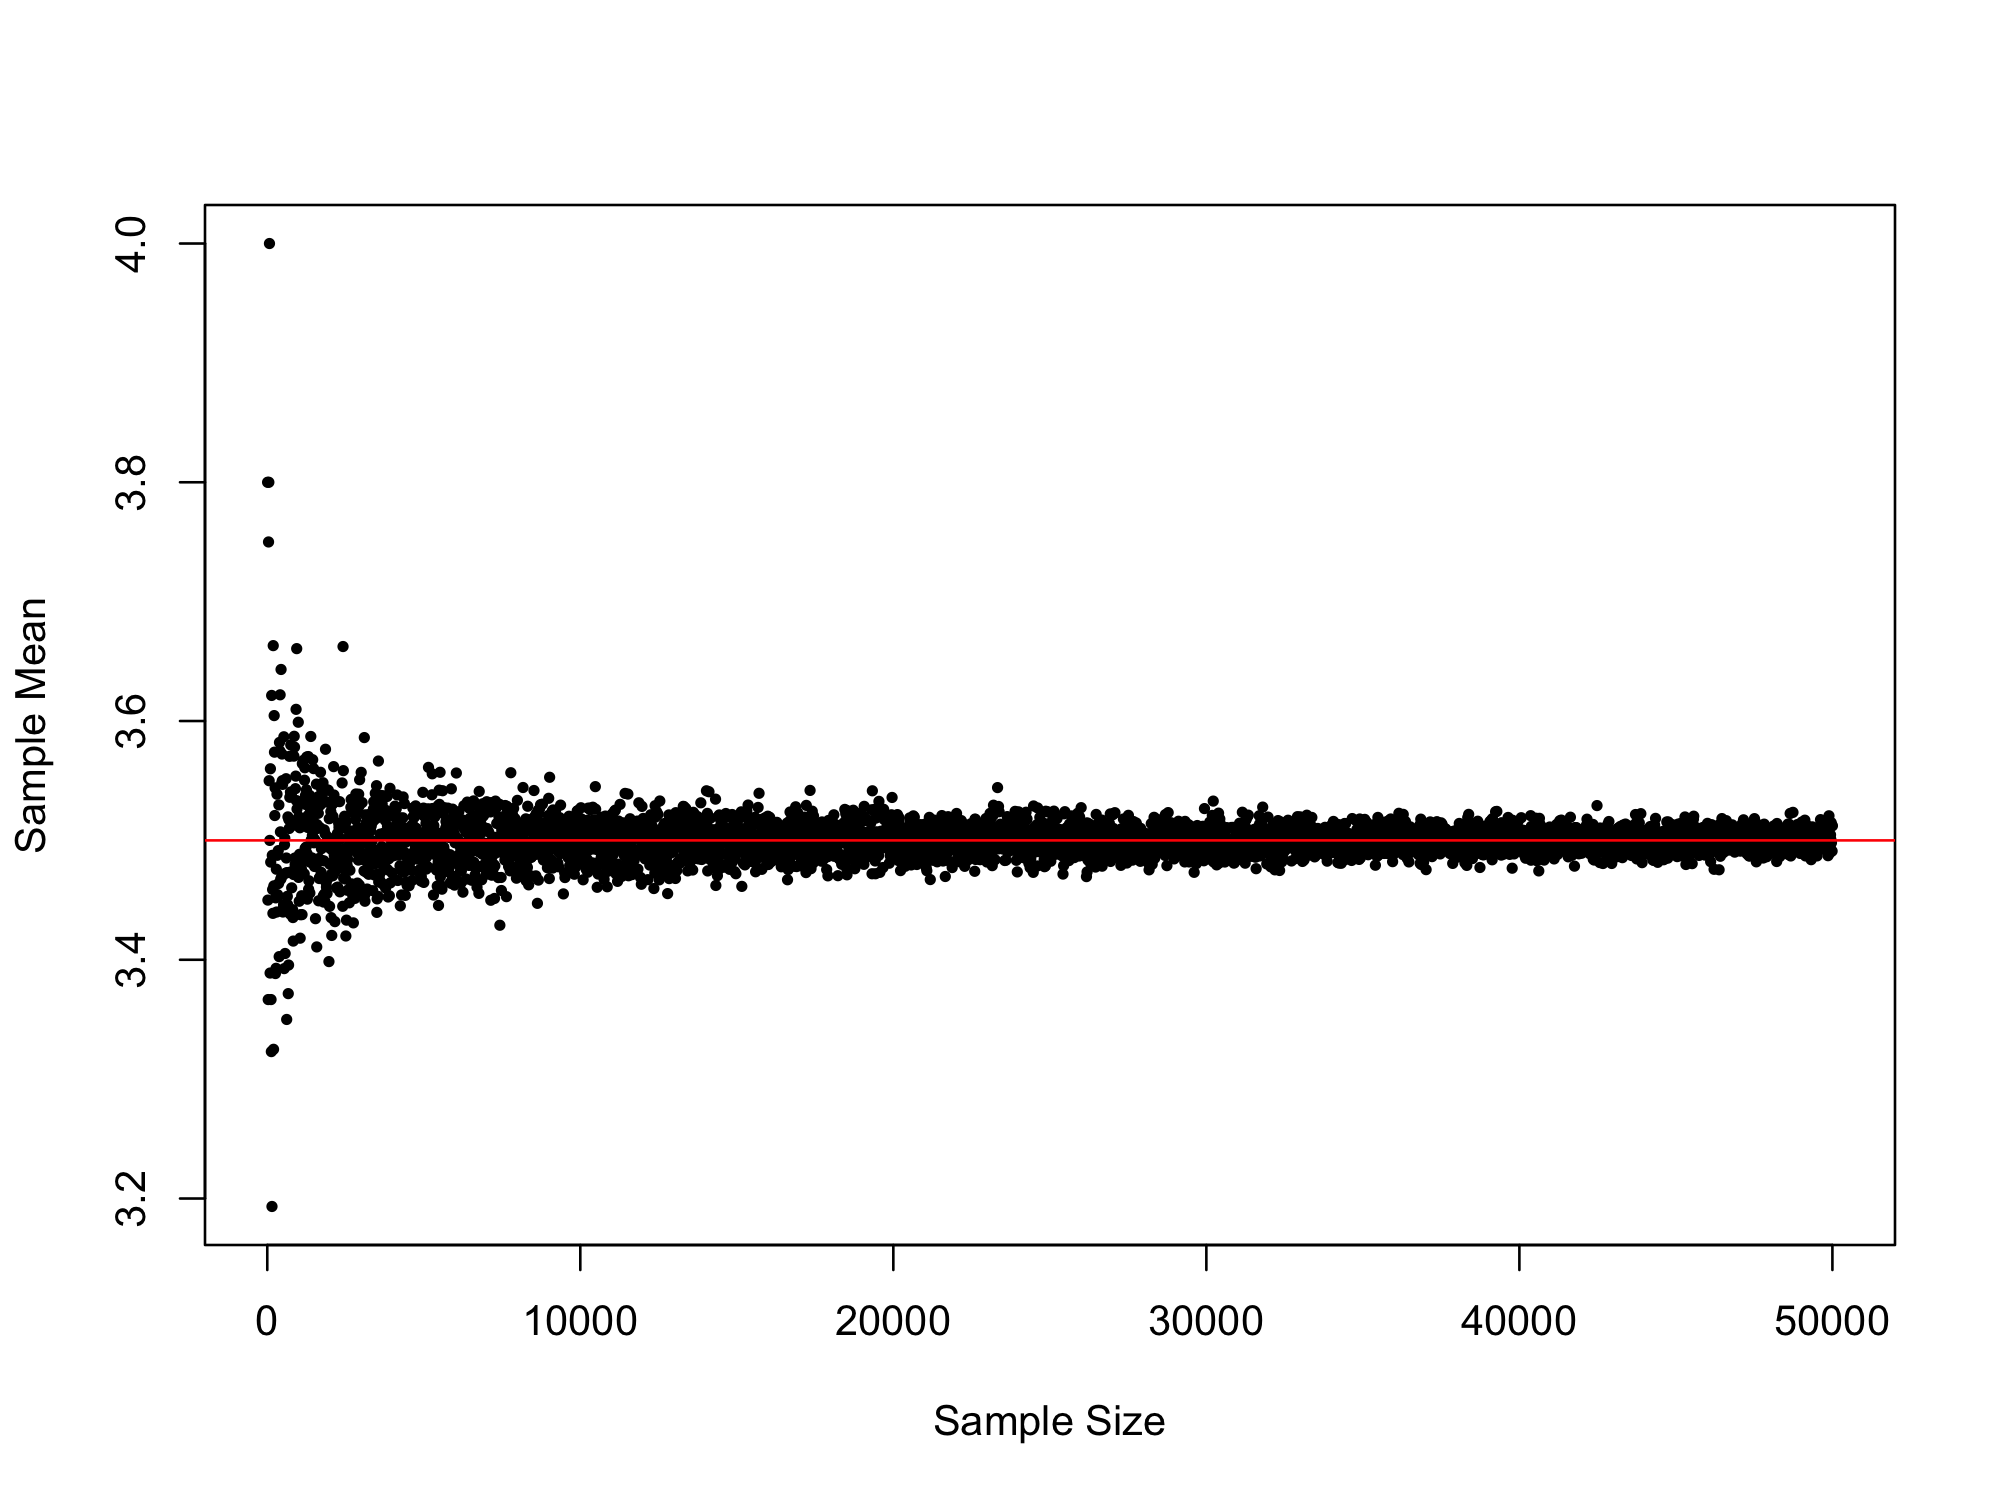
\includegraphics[scale=0.21]{img/die_plot}
		\captionof{figure}{Plot of Expected Value as sample grows}
		\label{fig:dieplot}
	\end{center}
\end{figure}



\section{Computing probabilities}

The law of large numbers gives a way to compute probabilities. An example of this application is the hat check problem \citep{scoville1966hat}. Let see as an example a class with $n = 20$ students and a professor who completely forgets the names and faces of all of them. Suppose he randomly hands back the midterm exams, let $p_{n}$ be the probability that no one receives their ow test back. It is known that as $n \rightarrow \infty$ one have $p_{n} \rightarrow e^{-1}$. 

It is generated a random permutation of the 20 exams, as a permutation of 20 numbers, and each random permutation is considered independent. The experiment is repeated 10 000 times as shown in the following code; it is used R software \citep{r}. The result gives an approximation to a probability of 0.3644, which is quite good for even n=20 with respect to the expected value of $e^{-1}$. 

\lstinputlisting[language=R, firstline=6, lastline=14]{code/hat_check.R}

\section{Application in trading}

The law of large numbers can be seen in the world of trading too. A clear example of this is given by \citet{bsl2020}. The author suggests that a large number of trades with a higher reward to risk ratio (Sharpe ratio) will tend to be more effective than a smaller number of trades.

Let assume a scenario with a relevant strategy where what matters is how much one will make when right and how much one lose when one is wrong when putting on a trade. In this situation, basis the law of large numbers, a trade can be wrong the majority of the time but still be profitable.

Backtesting on the longest period possible gets one closer to the mean annualized returns. Let assume a backtested strategy with a true Sharpe ratio of 2. Trying this over a 40 day trading period (broadly around two months), and assuming a normal distribution with mean returns of $0.1\%$ one can see results in Figure \ref{fig:trades}, representing how the Sharpe ratios tend to be with an increasing number of trades. Histogram \ref{fig:15trades} shows with few trades that one would end up with a lesser Sharpe ratio than what was seen through backtesting and might observe more losses than wins. On the other hand, Histograms \ref{fig:500trades} and \ref{fig:2500trades} one can see as the trials keep increasing, the Sharpe ratio is tending towards the backtested number (by tending towards a normal distribution).

	
	 \begin{figure}
	\centering
	\begin{subfigure}[b]{0.45\textwidth}
		\centering
		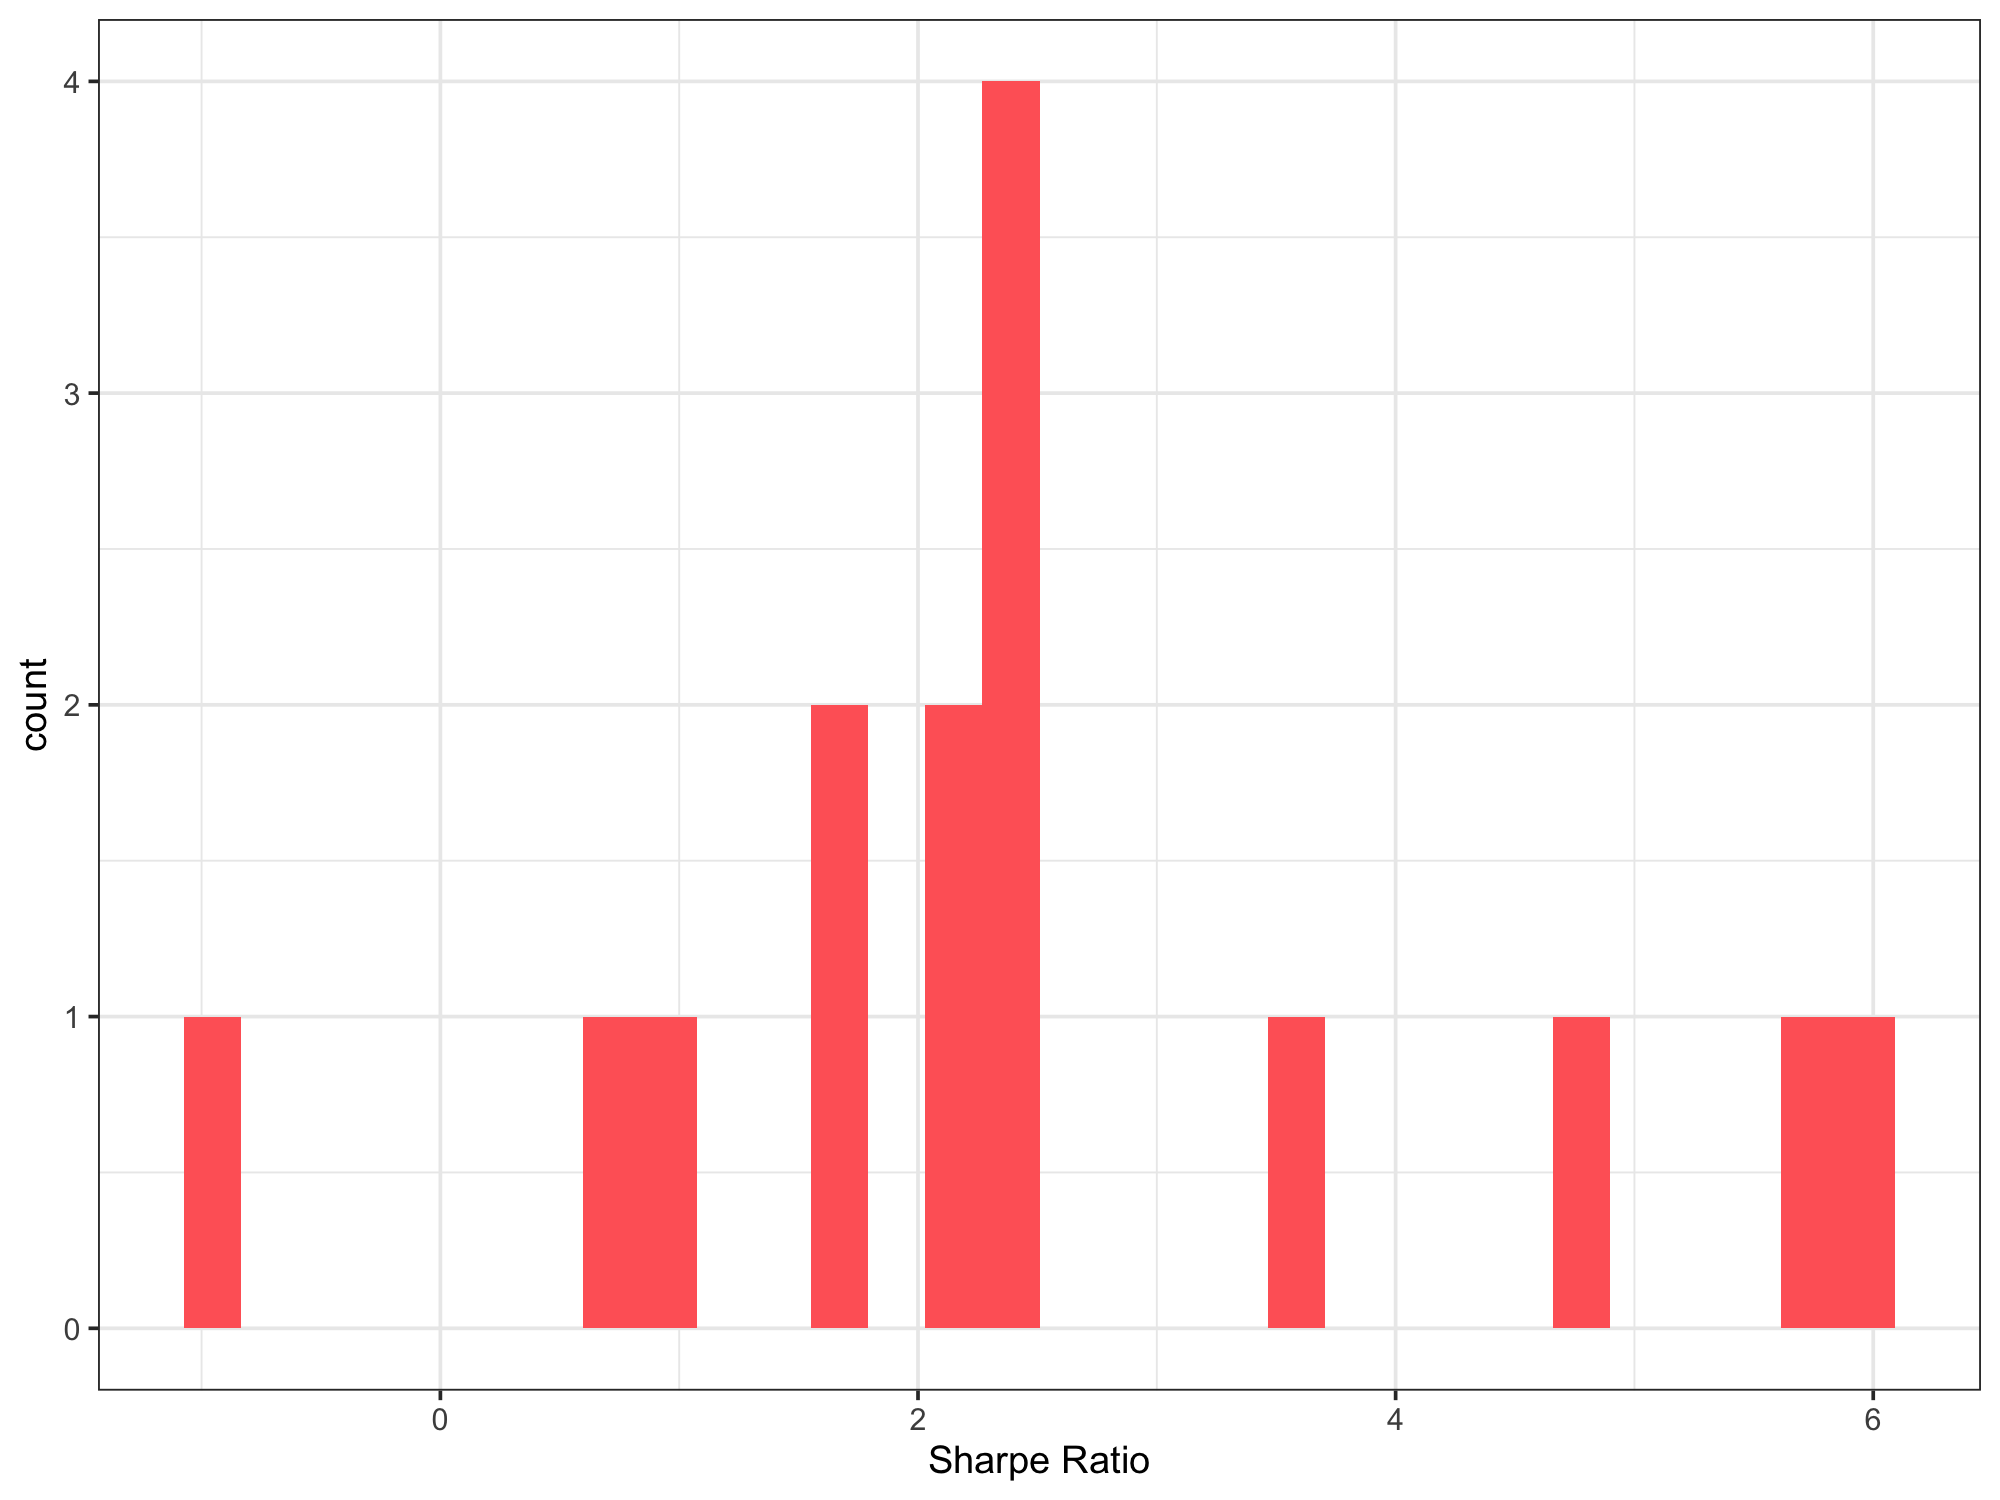
\includegraphics[width=\textwidth]{img/hist15}
		\caption[]%
		{{\small Histogram of 15 trades}}    
		\label{fig:15trades}
	\end{subfigure}
	\hfill
	\begin{subfigure}[b]{0.45\textwidth}  
		\centering 
		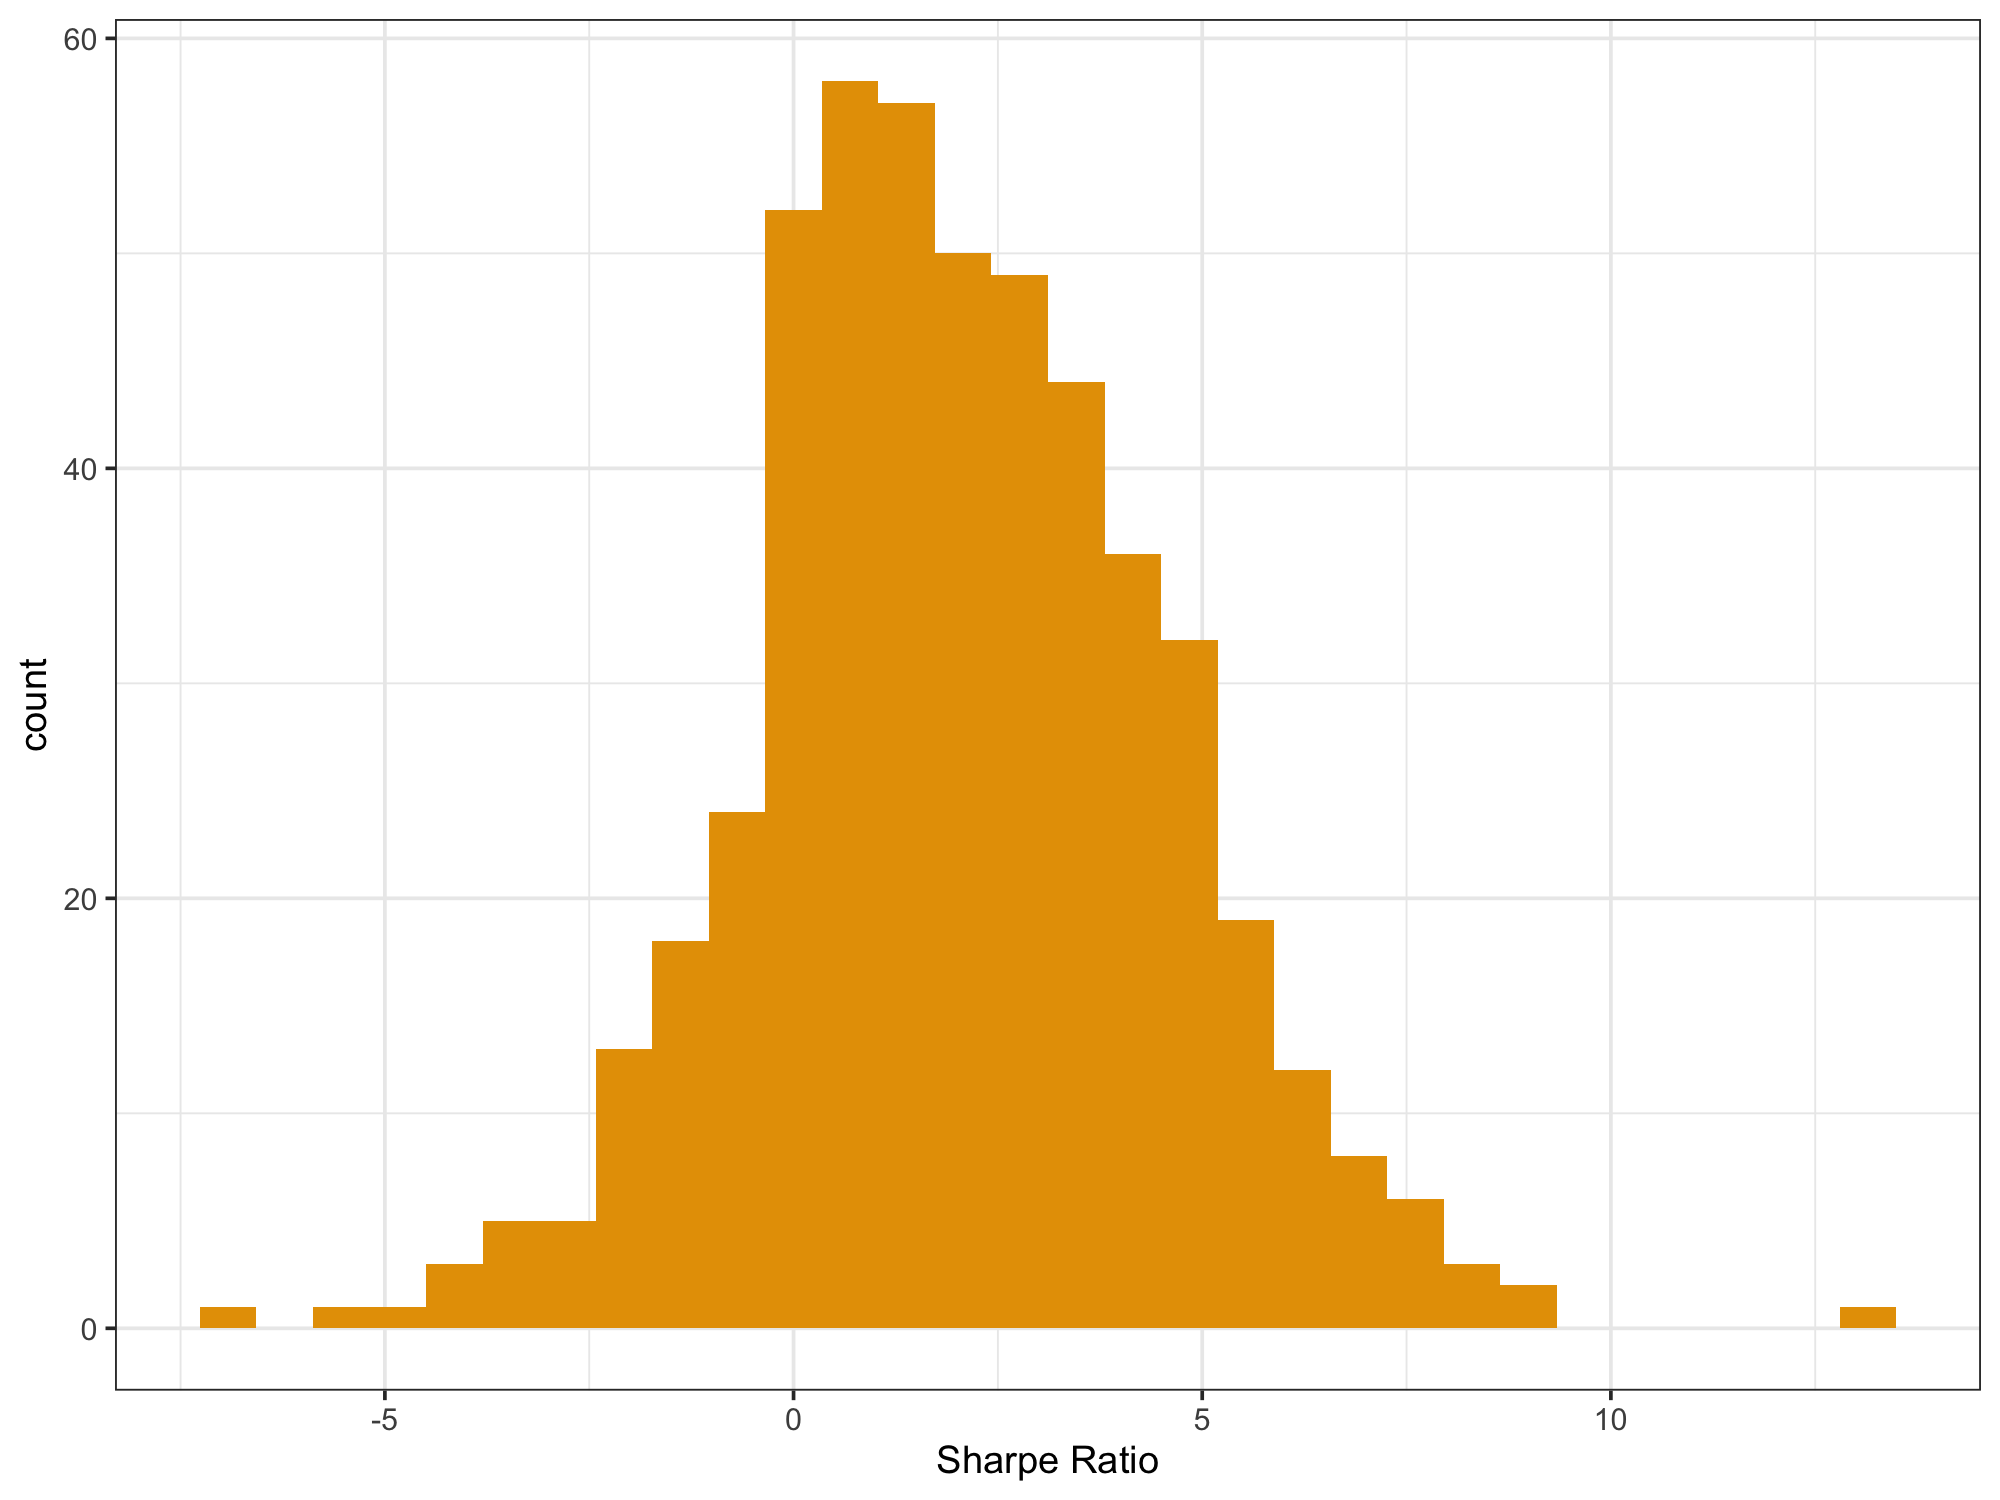
\includegraphics[width=\textwidth]{img/hist500}
		\caption[]%
		{{\small Histogram with 500 trades}}    
		\label{fig:500trades}
	\end{subfigure}
	\vskip\baselineskip
	\begin{subfigure}[b]{0.6\textwidth}   
		\centering 
		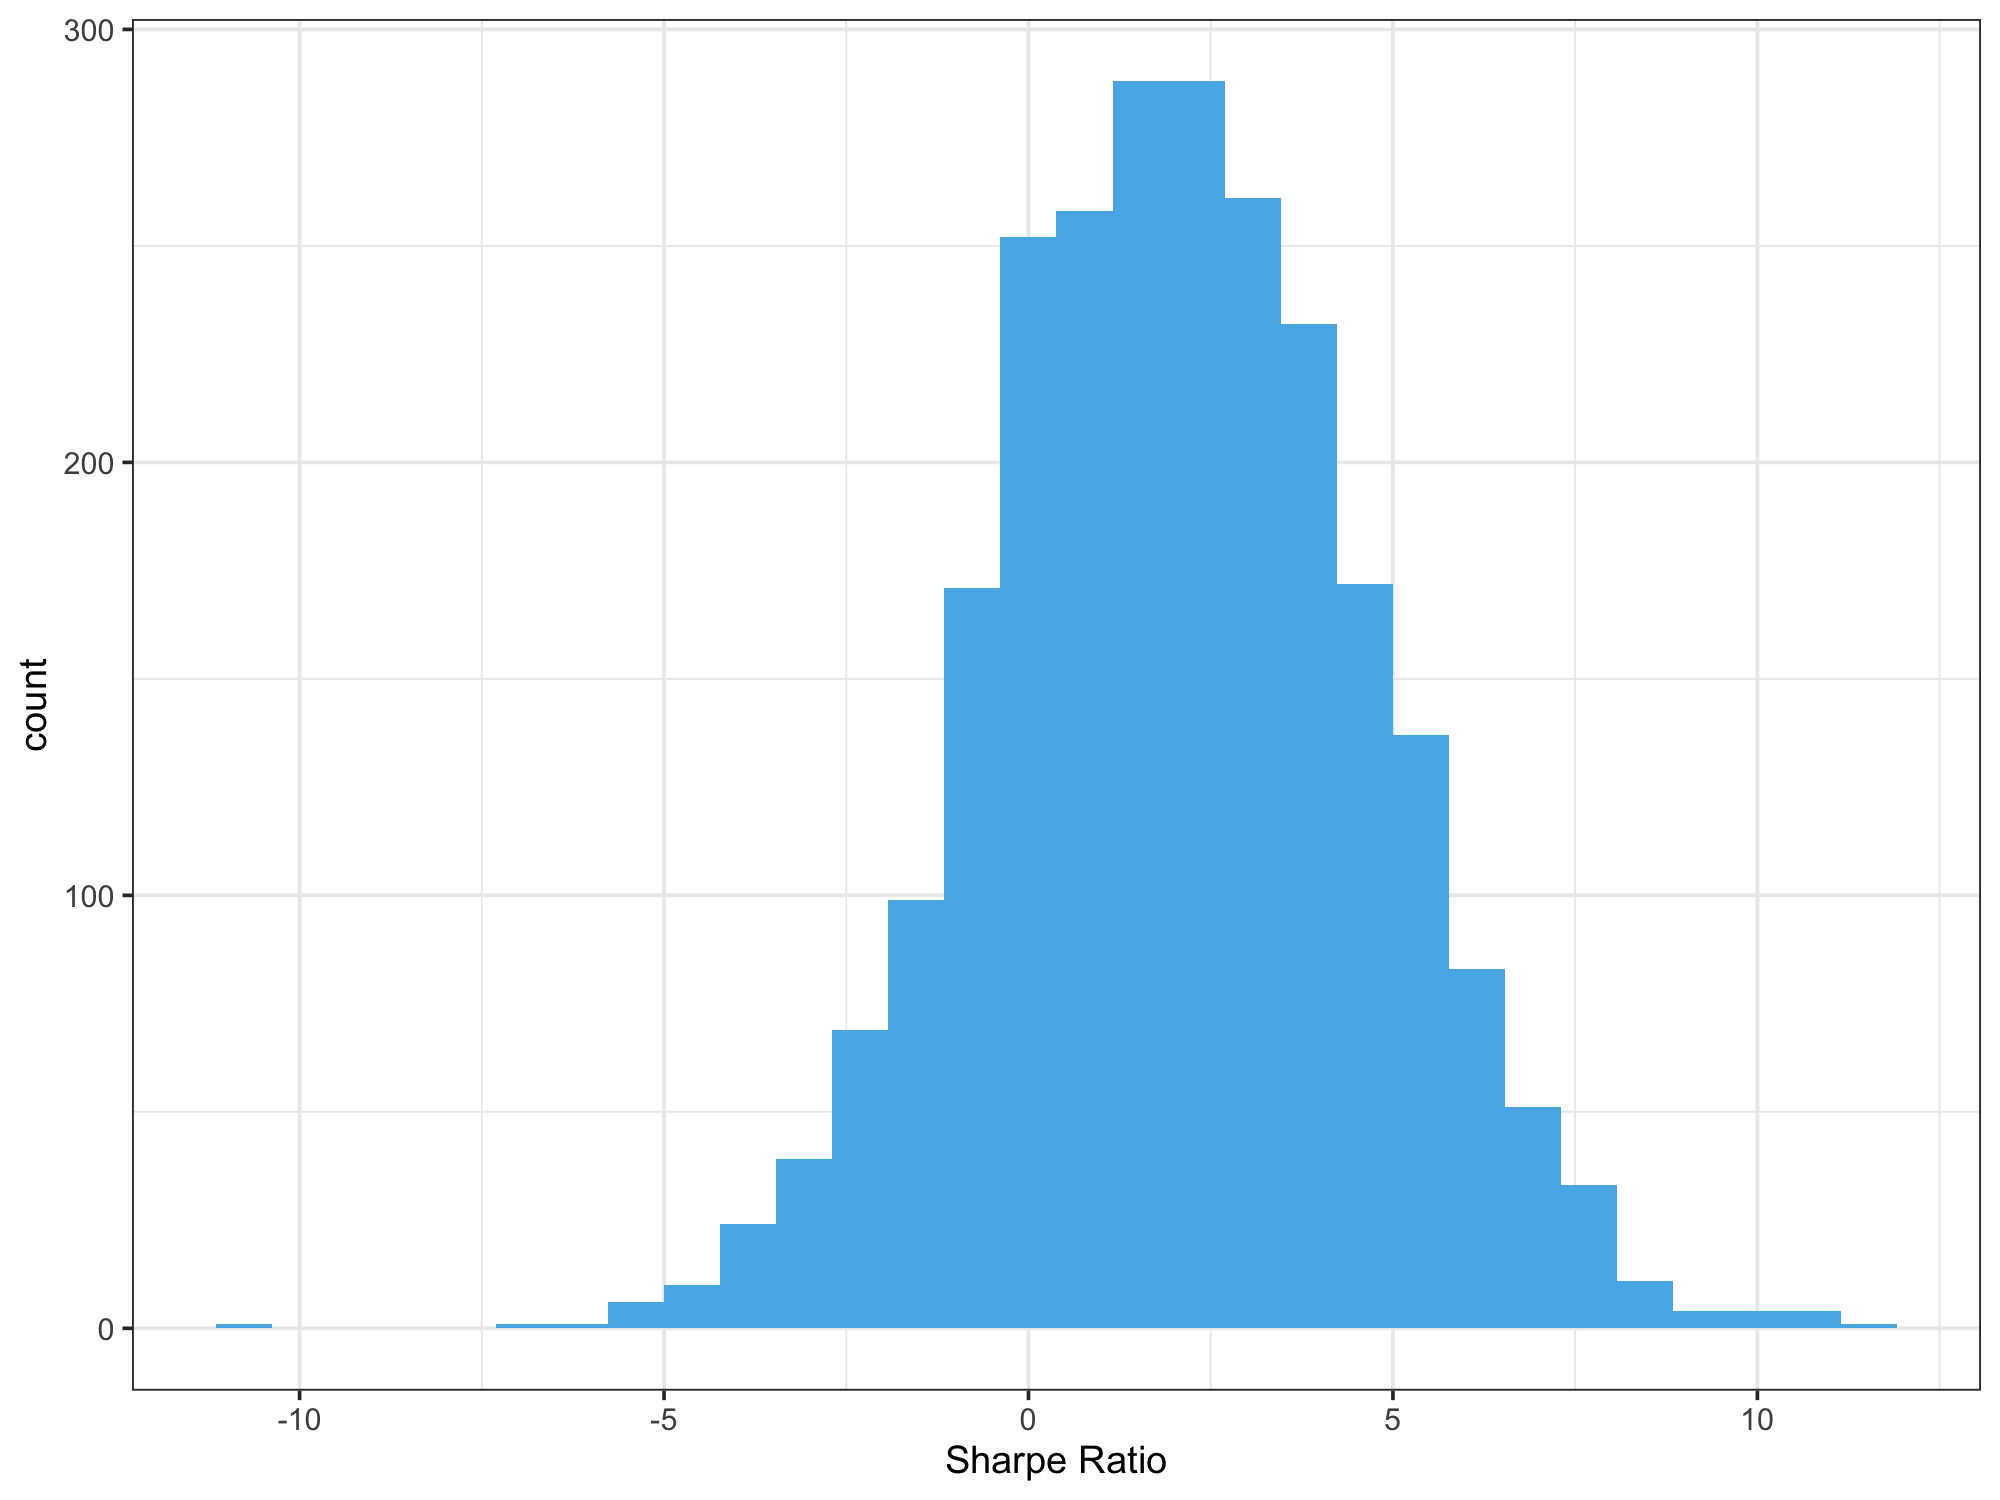
\includegraphics[width=\textwidth]{img/hist2500}
		\caption[]%
		{{\small Histogram of 2500 trades}}    
		\label{fig:2500trades}
	\end{subfigure}
\caption[ ]
{\small Histograms of the Sharpe ratios as the number of trades grows.} 
\label{fig:trades}
\end{figure}


		
\clearpage

	\bibliography{as13}
	\bibliographystyle{plainnat}
	
\end{document}

%https://statisticsglobe.com/sample-function-in-r/
%https://stackoverflow.com/questions/33373872/simple-simulation-of-the-law-of-large-numbers-lln-in-r
%https://sevragorgia.github.io/Research/r/statistics/Law-of-Large-Numbers/
%https://eranraviv.com/laws-of-large-numbers/
%https://umatter.github.io/courses/berkstats/Berkstats_LLM_CLT.html
%https://tsoo-math.github.io/ucl/prob-viaR.html